\chapter{Deployment}
\label{ch:deployment}
\section{Containerization}
% ** docker image for each microservice, docker file
% docker compose grouping containers and defining dependencies**

Data l'architettura del progetto in microservizi, usare Docker per creare un'immagine per ogni servizio è stata una scelta naturale. 
L'obiettivo finale è avere un sistema facilmente deployabile e scalabile, eseguibile velocemente in un ambiente generico, con uno stack di container Docker che racchiuda tutto il sistema.
Per fare ciò è stato necessario creare un Dockerfile per ogni servizio, in modo da poter creare un'immagine durante la fase di deploy della continuous integration.
\vspace{1cm}

La \textbf{strategia di containerizzazione} per tutte le immagini create è stata quella di utilizzare un'immagine base di Alpine, in modo da avere immagini leggere e veloci da scaricare. Per ridurre la dimensione delle immagini,
si è utilizzata un'immagine di sviluppo per compilare il codice e un'immagine di produzione per eseguire il codice compilato, copiando solo i file necessari.

\begin{figure}[H]
\caption{Comparazione tra le immagini multi-stage e le immagini tradizionali}
\centering
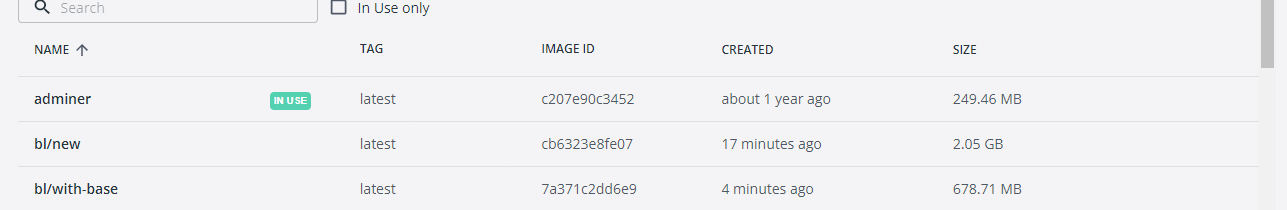
\includegraphics[width=12cm]{report/img/multi_stage.png}\\[5.5cm]
\end{figure}

\subsection{NodeJS}

I servizi UserManagementMaraffa e BusinessLogic sono stati containerizzati utilizzando un'immagine di Node.js. Nell'esempio sotto, si può notare la distinzione tra i diversi stage.
\vspace{1cm}

\begin{lstlisting}[language=Python, caption={Dockerfile delle immagini NodeJS}, label=list:dockerfile_nodejs]
FROM node:20-alpine as base
WORKDIR /app
COPY yarn.lock package.json /app/
RUN yarn install
COPY . /app
RUN yarn build

FROM node:20-alpine
WORKDIR /app    
COPY --from=base /app/package.json /app/package.json
COPY --from=base /app/node_modules /app/node_modules
COPY --from=base /app/dist /app/dist
EXPOSE 3000
CMD ["node","dist/main.js"]
\end{lstlisting}

\subsection{Java}

La containerizzazione del middleware ha richiesto alcuni passaggi aggiuntivi rispetto ai servizi in Node.js.
È stato necessario adottare immagini diverse per gli stage di build e produzione, quindi usare un'immagine di Gradle per la build, nella quale eseguire i comandi di Gradle, e un'immagine di 
OpenJDK per l'esecuzione del JAR prodotto dalla build.

Per la compilazione con Gradle, nonostante non sia una pratica corretta, è stato necessario mantenere nella repository il file gradle-wrapper.jar, in quanto non era possibile scaricarlo durante la build all'interno delle GitHub Actions.
La build non utilizza il classico comando di Gradle per generare il file .jar, ma un task personalizzato che si occupa di generare il fatJar del servizio, poiché le dipendenze non venivano gestite correttamente all'interno del normale file .jar.

\begin{lstlisting}[language=Java, caption={Task del fatJar da includere nel container}, label=list:gradle_fatJar]
tasks.register<Jar>("fatJar") {
    archiveBaseName.set("Middleware")
    manifest {
        attributes["Main-Class"] = "server.Main"
    }
    from(sourceSets.main.get().output)
    dependsOn(configurations.runtimeClasspath)
    from({ configurations.runtimeClasspath.get().filter { it.name.endsWith("jar") }.map { zipTree(it) } })
    dependsOn("compileJava")
    duplicatesStrategy = DuplicatesStrategy.EXCLUDE // Puoi utilizzare altre strategie come DuplicatesStrategy.WARN per avvisare ma non fermare la build
}
\end{lstlisting}

\subsection{Angular}

La containerizzazione del frontend ha richiesto l'utilizzo di un'immagine di Node.js per lo stage di build, mentre per l'esecuzione è stata utilizzata un'immagine di Nginx.
Come citato nella sezione \ref{Nginx} Nginx serve per eseguire l'applicazione all'interno del container e per poterla raggiungere dall'esterno.

\section{Monitoraggio}

In un progetto composto da microservizi deployati con container, il monitoraggio è essenziale per garantire il corretto funzionamento e la performance ottimale del sistema. Per realizzare un monitoraggio efficace dei container, sono stati impiegati i container di Grafana, Prometheus e cAdvisor.

\subsection{Grafana}

Grafana è uno strumento open-source per la visualizzazione e l'analisi delle metriche raccolte. Viene utilizzato per creare dashboard personalizzate che mostrano lo stato e le performance dei microservizi. Con Grafana, è possibile configurare alert che notificano immediatamente eventuali problemi nel sistema, permettendo una risposta rapida e mirata.

\subsection{Prometheus}

Prometheus è un sistema di monitoraggio e di allarme progettato per raccogliere e memorizzare metriche in serie temporali. È stato configurato per raccogliere metriche dai container dei microservizi e da cAdvisor. Prometheus esegue la raccolta dei dati a intervalli regolari e li memorizza in un database time-series, rendendoli disponibili per l'analisi e la visualizzazione in Grafana.

\subsection{cAdvisor}

cAdvisor (Container Advisor) è uno strumento che fornisce informazioni sulle risorse utilizzate dai container, come CPU, memoria, rete e disco. È stato integrato con Prometheus per raccogliere e esportare le metriche dei container. cAdvisor offre una visione dettagliata delle performance di ogni container, aiutando a identificare e risolvere problemi di utilizzo delle risorse.

\subsection{Integrazione e Configurazione}

L'integrazione di Grafana, Prometheus e cAdvisor ha permesso di creare un sistema di monitoraggio completo. I container di cAdvisor raccolgono le metriche di utilizzo delle risorse dai container dei microservizi e le esportano a Prometheus. Prometheus memorizza queste metriche e le rende disponibili per la visualizzazione in Grafana. Le dashboard di Grafana sono configurate per mostrare le metriche chiave e fornire un'analisi dettagliata dello stato del sistema.

La configurazione di questi strumenti è stata gestita tramite Docker Compose, permettendo una facile implementazione e scalabilità del sistema di monitoraggio. Le variabili d'ambiente e i file di configurazione sono stati impostati per garantire la corretta connessione e funzionamento dei container di monitoraggio.

\begin{lstlisting}[language=Python, caption={Esempio di configurazione Docker Compose}, label=list:docker_compose_monitoring]
 cadvisor:
    container_name: cadvisor
    image: gcr.io/cadvisor/cadvisor:latest
    ports:
      - "8080:8080"
    volumes:
      - "/:/rootfs"
      - "/var/run:/var/run"
      - "/sys:/sys"
      - "/var/lib/docker/:/var/lib/docker"
      - "/dev/disk/:/dev/disk"
    privileged: true
    devices:
      - "/dev/kmsg"

  prometheus:
    container_name: prometheus
    image: prom/prometheus:latest
    ports:
      - "9090:9090"
    volumes:
      - "./prometheus.yml:/etc/prometheus/prometheus.yml"
    privileged: true
    depends_on:
      - cadvisor

  grafana:
    container_name: grafana
    image: grafana/grafana:latest
    ports:
      - "3000:3000"
    environment:
      - GF_PATHS_PROVISIONING=/etc/grafana/provisioning
      - DS_PROMETHEUS=prometheus
    volumes:
      - "grafana-data:/var/lib/grafana"
      - "./datasources.yml:/etc/grafana/provisioning/datasources/datasources.yml"
      - "./dashboard.json:/var/lib/grafana/dashboards/dashboard.json"
      - "./default.yaml:/etc/grafana/provisioning/dashboards/default.yaml"
    privileged: true
    depends_on:
      - prometheus
\end{lstlisting}

Con questa configurazione, il sistema di monitoraggio offre una visione completa delle performance e dello stato dei microservizi, permettendo di mantenere un'operatività ottimale e di intervenire prontamente in caso di anomalie.
